%
% Assignment Template
% Last modified 9/11/2024 by Ziyong Wang

\documentclass[11pt]{article}
\usepackage[left=0.7in,right=0.7in,top=1in,bottom=0.7in]{geometry}
\usepackage{fancyhdr} % for header
\usepackage{graphicx} % for figures
\usepackage{amsmath}  % for extended math markup
\usepackage{amssymb}
\usepackage{inconsolata}
\usepackage{enumitem}
\usepackage[bookmarks=false]{hyperref} % for URL embedding
\usepackage[noend]{algpseudocode} % for pseudocode
\usepackage[plain]{algorithm} % float environment for algorithms

%%%%%%%%%%%%%%%%%%%%%%%%%%%%%%%%%%%%%%%%%%%%%%%%%%%%%%%%%%%%%%%%%%%%%%

\newcommand{\StudentName}{Ziyong Wang}
\newcommand{\StudentID}{522790}
\newcommand{\HomeworkNumber}{2}

%%%%%%%%%%%%%%%%%%%%%%%%%%%%%%%%%%%%%%%%%%%%%%%%%%%%%%%%%%%%%%%%%%%%%%%%

% create header and footer for every page
\pagestyle{fancy}
\fancyhf{}
\lhead{\textbf{\StudentName}}
\chead{\textbf{\StudentID}}
\rhead{\textbf{Assignment \HomeworkNumber}}
\cfoot{\thepage}

% preferred pseudocode style
\algrenewcommand{\algorithmicprocedure}{}
\algrenewcommand{\algorithmicthen}{}

% ``do { ... } while (cond)''
\algdef{SE}[DOWHILE]{Do}{doWhile}{\algorithmicdo}[1]{\algorithmicwhile\ #1}%

% ``for (x in y ... z)''
\newcommand{\ForRange}[3]{\For{#1 \textbf{in} #2 \ \ldots \ #3}}

% these are common math formatting commands that aren't defined by default
\newcommand{\union}{\cup}
\newcommand{\isect}{\cap}
\newcommand{\ceil}[1]{\ensuremath \left\lceil #1 \right\rceil}
\newcommand{\floor}[1]{\ensuremath \left\lfloor #1 \right\rfloor}

%%%%%%%%%%%%%%%%%%%%%%%%%%%%%%%%%%%%%%%%%%%%%%%%%%%%%%%%%%%%%%%%%%%%%%

\begin{document}

% text goes here!

\begin{enumerate}
    \item $$
    \begin{aligned}
        \Pr(x=6 | n=10) &= \Pr(x=6 |\theta = \frac{1}{2}, n=10) Pr(\theta = \frac{1}{2}) + \int_{\theta \neq \frac{1}{2}} \Pr(x=6 | \theta, n=10) p(\theta) d\theta \\
        &= {10 \choose 6} {\frac{1}{2}}^{10} \frac{1}{2} + \int_{\theta \neq \frac{1}{2}} {10 \choose 6} \theta^6 (1-\theta)^4 \frac{1}{2} d\theta\\
        &= \frac{1}{2} {10 \choose 6} \left(\frac{1}{1024} + \frac{1}{2310}\right)\\
        \Pr(\theta = \frac{1}{2} | x=6, n=10) &= \frac{\Pr(x=6 | \theta = \frac{1}{2}, n=10)\Pr(\theta = \frac{1}{2})}{\Pr(x=6 | n=10)} = \frac{\frac{1}{2} {10 \choose 6} \frac{1}{1024}}{\frac{1}{2} {10 \choose 6} \left(\frac{1}{1024} + \frac{1}{2310}\right)} = 0.693 \\
        p(\theta | x=6, n=10) &= \frac{p(x=6 | \theta, n=10)p(\theta)}{\Pr(x=6 | n=10)} = \frac{\frac{1}{2} {10 \choose 6} \theta^6 (1-\theta)^4}{\frac{1}{2} {10 \choose 6} \left(\frac{1}{1024} + \frac{1}{2310}\right)} = 709.5\theta^6 (1-\theta)^4 \\
    \end{aligned}
    $$

    \item 
    \begin{enumerate}[label=(\alph*)]
        \item The posterior distribution is $p(\theta | \mathcal{D}) = \mathcal{B}(901, 101)$, the posterior mean is $\mathbb{E}[\theta | \mathcal{D}] = \frac{901}{1002}$.
        \item The posterior distribution is $p(\theta | \mathcal{D}) = \mathcal{B}(901, 200)$, the posterior mean is $\mathbb{E}[\theta | \mathcal{D}] = \frac{901}{1101}$.
        \item The posterior mean is $\mathbb{E}[\theta | \mathcal{D}] = 0.4991$.
    \end{enumerate}

    \begin{figure}[h]
        \centering
        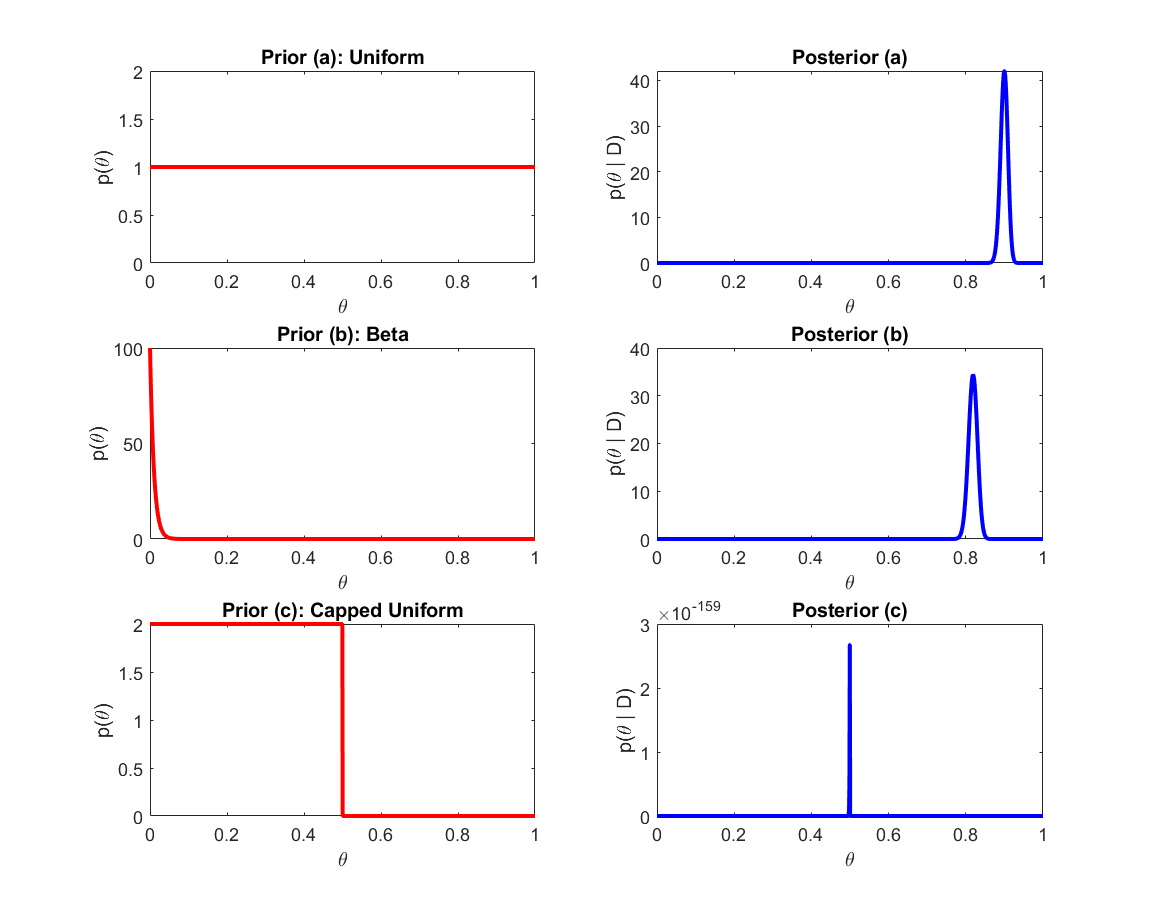
\includegraphics[width=1.\textwidth]{Question 2.png}
    \end{figure}
    
    \item $$
    \begin{aligned}
        \mathbb{E}[l(\hat{\theta}, \theta); c] 
        &= \int_{-\infty}^{\hat{\theta}} c \cdot p(\theta) d \theta + \int_{\hat{\theta}}^{\infty} (\theta - \hat{\theta})^2 p(\theta) d \theta \\
        &= \frac{c}{\sqrt{2\pi}} \int_{-\infty}^{\hat{\theta}} e^{-\frac{\theta^2}{2}} d \theta + \frac{1}{\sqrt{2\pi}} \int_{\hat{\theta}}^{\infty} (\theta - \hat{\theta})^2 e^{-\frac{\theta^2}{2}} d \theta \\
        &= \frac{c}{2} \left(\operatorname{erf}\left(\frac{\hat{\theta}}{\sqrt{2}}\right) + 1\right) + \frac{\hat{\theta}^2 + 1}{2} \left(1-\operatorname{erf}\left(\frac{\hat{\theta}}{\sqrt{2}}\right)\right) - \frac{e^{-\hat{\theta}^2/2}\hat{\theta}}{\sqrt{2\pi}} \\
        &= \frac{\hat{\theta}^2+c+1}{2} - \frac{\hat{\theta}^2-c+1}{2} \operatorname{erf}\left(\frac{\hat{\theta}}{\sqrt{2}}\right)- \frac{e^{-\hat{\theta}^2/2}\hat{\theta}}{\sqrt{2\pi}}
    \end{aligned}
    $$

    where $\operatorname{erf}(x)=\frac{2}{\sqrt{\pi}} \int_{0}^{x} e^{-t^2} dt$ is the error function.

    The first order derivatives are
    $$
    \begin{aligned}
        \frac{\partial \mathbb{E}[l(\hat{\theta}, \theta); c]}{\partial \hat{\theta}}
        &= \hat{\theta} - \hat{\theta} \operatorname{erf}\left(\frac{\hat{\theta}}{\sqrt{2}}\right) - \frac{\hat{\theta}^2-c+1}{2} \frac{2}{\sqrt{\pi}} e^{-\hat{\theta}^2/2} \frac{1}{\sqrt{2}} - \frac{e^{-\hat{\theta}^2/2} - e^{-\hat{\theta}^2/2} \hat{\theta}^2}{\sqrt{2\pi}} \\
        &= \hat{\theta} - \hat{\theta} \operatorname{erf}\left(\frac{\hat{\theta}}{\sqrt{2}}\right) - \frac{2-c}{\sqrt{2\pi}}  e^{-\hat{\theta}^2/2} 
    \end{aligned}
    $$

    When the first order conditions are met, we have
    
    \begin{equation}
        \hat{\theta} - \hat{\theta} \operatorname{erf}\left(\frac{\hat{\theta}}{\sqrt{2}}\right) = \frac{2-c}{\sqrt{2\pi}}  e^{-\hat{\theta}^2/2}
    \end{equation}

    In this case, the second order derivatives are
    $$
    \begin{aligned}
        \frac{\partial^2 \mathbb{E}[l(\hat{\theta}, \theta); c]}{\partial \hat{\theta}^2}
        &= \frac{\partial}{\partial \hat{\theta}} \left[\hat{\theta} - \hat{\theta} \operatorname{erf}\left(\frac{\hat{\theta}}{\sqrt{2}}\right) - \frac{2-c}{\sqrt{2\pi}}  e^{-\hat{\theta}^2/2}\right] \\
        &= 1 - \operatorname{erf}\left(\frac{\hat{\theta}}{\sqrt{2}}\right) - \hat{\theta} \sqrt{\frac{2}{\pi}} e^{-\hat{\theta}^2/2} + \frac{2-c}{\sqrt{2\pi}}  e^{-\hat{\theta}^2/2} \hat{\theta} \\
        &= 1 - \operatorname{erf}\left(\frac{\hat{\theta}}{\sqrt{2}}\right) - \frac{c\hat{\theta}}{\sqrt{2\pi}} e^{-\hat{\theta}^2/2} \\
        &= \left(1 - \operatorname{erf}\left(\frac{\hat{\theta}}{\sqrt{2}}\right)\right) \left(1 - \frac{c\hat{\theta}}{\sqrt{2\pi}} \frac{\sqrt{2\pi}\hat{\theta}}{2-c}\right) \\
        &= \left(1 - \operatorname{erf}\left(\frac{\hat{\theta}}{\sqrt{2}}\right)\right) \left(1 - \frac{c\hat{\theta}^2}{2-c}\right)
    \end{aligned}
    $$
    
    Note that the error function is always smaller than 1, the second order conditions means that

    \begin{equation}
        \frac{c\hat{\theta}^2}{2-c} < 1
    \end{equation}
    
    When $c>2$,

    $$
        \frac{c\hat{\theta}^2}{2-c} < 0
    $$

    When $c<2$, 

    $$
        \hat{\theta} \left(1 - \operatorname{erf}\left(\frac{\hat{\theta}}{\sqrt{2}}\right)\right) = \frac{2-c}{\sqrt{2\pi}}  e^{-\hat{\theta}^2/2} > 0
    $$
    
    which means that $\hat{\theta} > 0$. In this case,  the second order condition implies
    
    \begin{equation}
        0 < \hat{\theta} < \sqrt{\frac{2-c}{c}}
    \end{equation}

    To sum up, the Bayesian estimator is the $\hat{\theta}$ which satisfies $(1)$. It also satisfies $(3)$ when $c<2$.

    \begin{figure}[h]
        \centering
        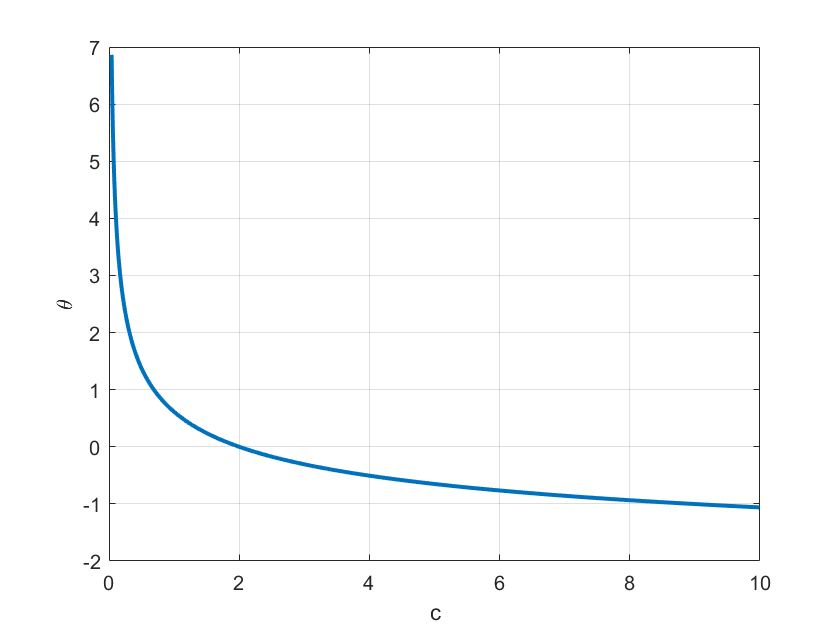
\includegraphics[width=1.\textwidth]{Question 3.png}
    \end{figure}
    
\end{enumerate}

\end{document}
